\documentclass[10pt,a4paper]{report}
\usepackage[latin1]{inputenc}
\usepackage{amsmath}
\usepackage{amsfonts}
\usepackage{amssymb}
\usepackage{graphicx}
\usepackage{subfig}
\usepackage[export]{adjustbox}
\usepackage{placeins}
\author{Michael C. Kunkel}
\newlength{\figwidth}
\setlength{\figwidth}{0.9\columnwidth}

\newlength{\qfigheight}
\setlength{\qfigheight}{0.25\textheight}

\newlength{\hfigheight}
\setlength{\hfigheight}{0.5\textheight}
\begin{document}
	To calculate the track-efficiency systematic uncertainty, the calculation was redone as described in Sec. 6.2 of the analysis note. The track-efficiency for the systematic study had a binning scheme of $\theta$, $\phi$, Fig.~\ref{fig:toteff_protnew}, instead of the $\theta \sin\phi$, $\theta \cos\phi$ binning seen in Fig. 31 in the analysis note.
	
\begin{figure}[h!]\begin{center}
		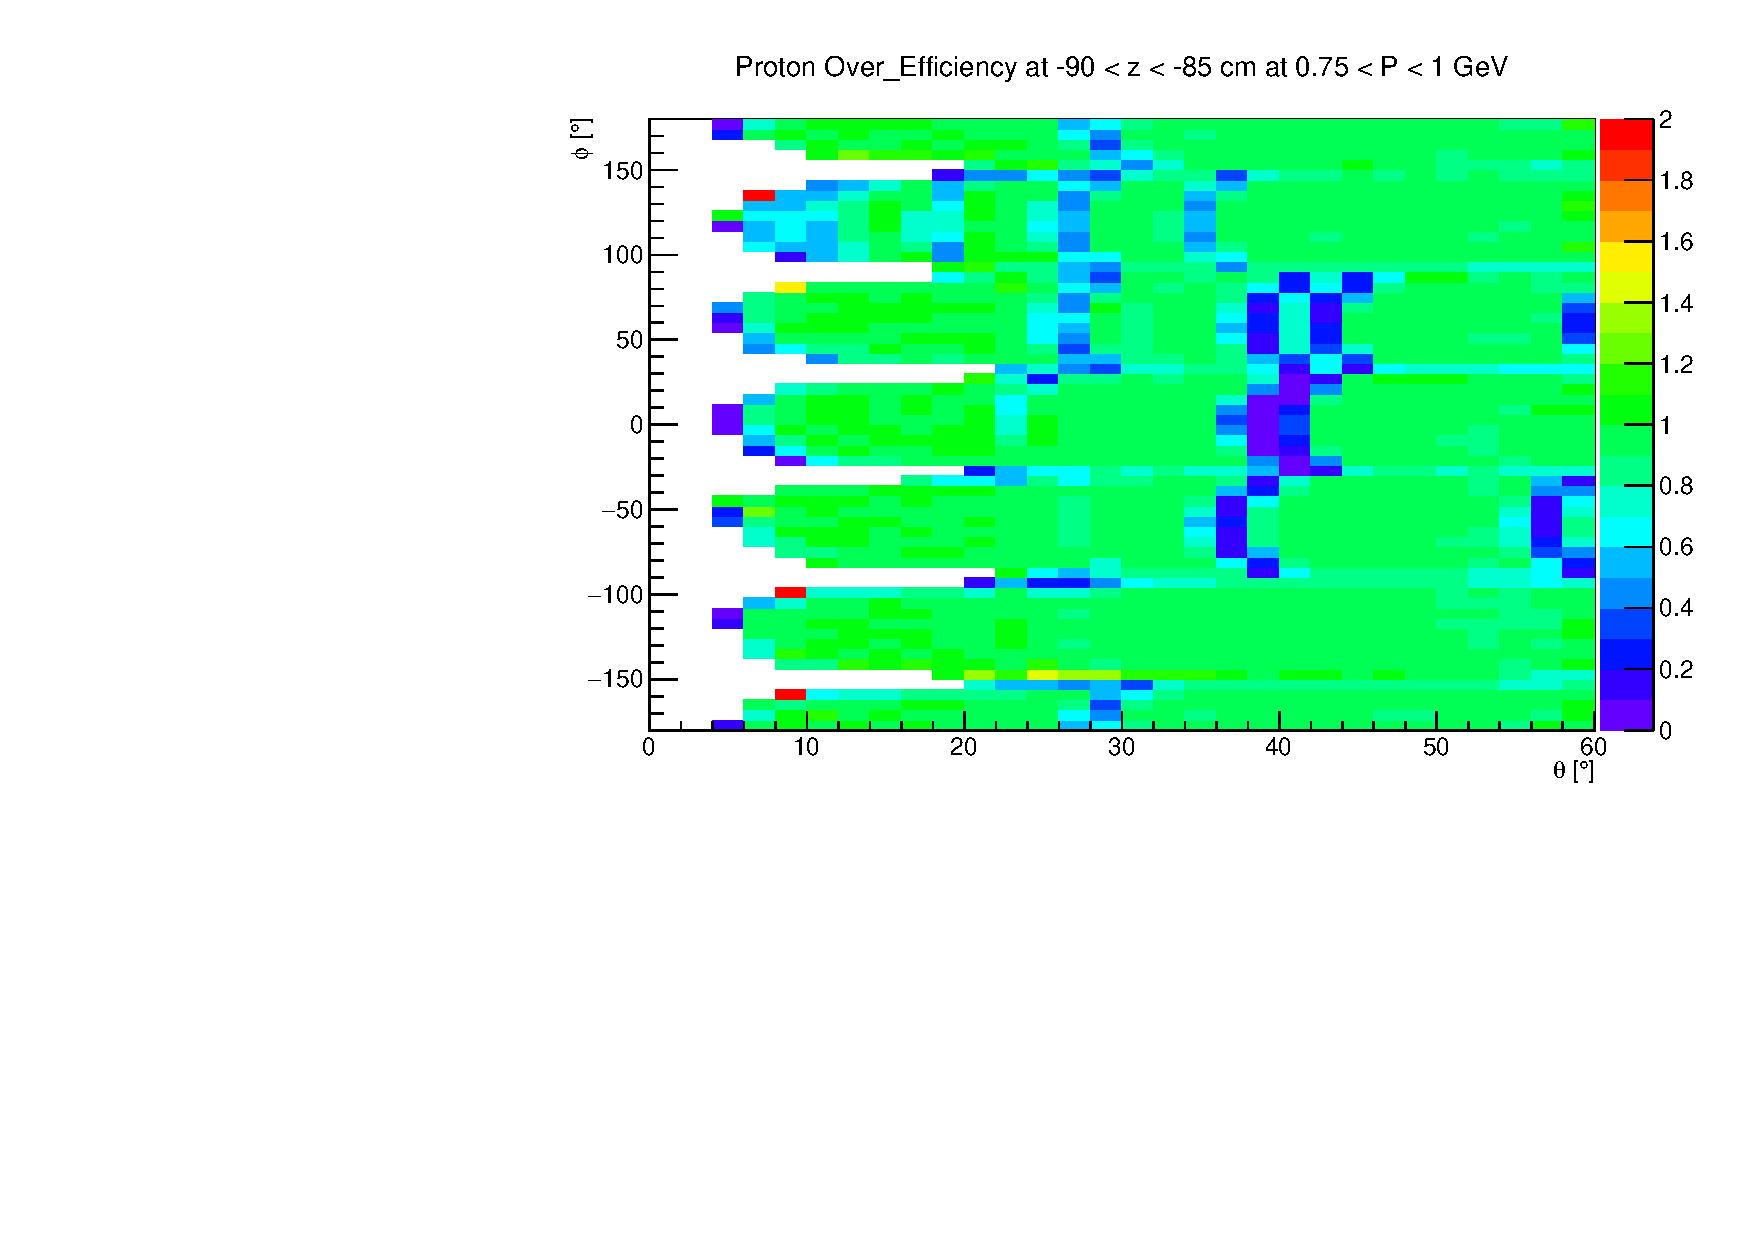
\includegraphics[width=1.1 \figwidth,height=\hfigheight]{/Users/michaelkunkel/WORK/GIT_HUB/Pi0_Papers/ANALYSIS_NOTE/RESULTS/NewEffPlot.pdf}
		\caption[$\phi$ vs. $\theta$ plot showing the over-efficiency of simulating the proton with z-vertex $-90\textless z\textless-85$~cm and momentum $0.75\textless p \textless 1$~GeV from a 2 charged track reaction]{\label{fig:toteff_protnew} $\phi$ vs. $\theta$ plot showing the over-efficiency of simulating the proton with z-vertex $-90\textless z\textless-85$~cm and momentum $0.75\textless p \textless 1$~GeV from a 2 charged track reaction.}
\end{center}\end{figure}
		
Three-charged track-efficiency values from the initial procedure, described in Sec. 6.2, were compared to the values from this new binning. Since both techniques are not known quantities, the method for calculating the error between the is;
\begin{align}
	\Delta = \frac{x_{previous} -x_{new} }{\frac{x_{previous} +x_{new}}{2}} \label{eq:eq1}
\end{align}	
where $x_{previous}$ is a value of a three-charged track-efficiency from the mapping of Sec~6.2 and $x_{new}$ is a three-charged track-efficiency from the mapping from the new set of figures derived for this systematic calculation.

Since both values are corrections, it makes little statistical sense to promote one to a "known value", therefore the only appropriate method to measure the error between the values is to use the percent difference method. In this method the denominator is the average value between the two hypotheses, hence the factor of 2.
\subsection*{Angular  dependence}
To investigate whether there exists a C.M.~$\cos \theta$ dependence, the values of Eq.~\ref{eq:eq1} were binned in according with the event C.M. $\cos \theta$, per $E_{\gamma}$ value.
\begin{figure}%
	\centering
	\subfloat[$-0.859<\cos \theta<-0.484$] {{\includegraphics[width=15cm,height=0.8 \hfigheight]{/Users/michaelkunkel/WORK/CLAS/CLAS6/CODES/SVN/clas/PI0/EFFICIENCY/CosProfiledHistMeanPartial_I.pdf} }}%
	
	\subfloat[$-0.391<\cos \theta<-0.031$] {{\includegraphics[width=15cm,height=0.8 \hfigheight]{/Users/michaelkunkel/WORK/CLAS/CLAS6/CODES/SVN/clas/PI0/EFFICIENCY/CosProfiledHistMeanPartial_II.pdf} }}%
	\caption{(Color Online)Mean relative uncertainty vs. $E_{\gamma}$ calculated between the two sets of track efficiencies for $\cos \theta$.}%
	\label{fig:example1}%
\end{figure}		
\begin{figure}%
	\centering
	\subfloat[$0.016<\cos \theta<0.141$]
	{\includegraphics[width=15cm,height=0.8 \hfigheight]{/Users/michaelkunkel/WORK/CLAS/CLAS6/CODES/SVN/clas/PI0/EFFICIENCY/CosProfiledHistMeanPartial_III.pdf} }%

	\subfloat[$0.172<\cos \theta<0.297$] {\includegraphics[width=15cm,height=0.8 \hfigheight]{/Users/michaelkunkel/WORK/CLAS/CLAS6/CODES/SVN/clas/PI0/EFFICIENCY/CosProfiledHistMeanPartial_IV.pdf} }%
	\caption{(Color Online)Mean relative uncertainty vs. $E_{\gamma}$ calculated between the two sets of track efficiencies for $\cos \theta$.}%
	\label{fig:example2}%
\end{figure}	
\begin{figure}%
	\centering
	\subfloat[$0.328<\cos \theta<0.453$] {{\includegraphics[width=15cm,height=0.8 \hfigheight]{/Users/michaelkunkel/WORK/CLAS/CLAS6/CODES/SVN/clas/PI0/EFFICIENCY/CosProfiledHistMeanPartial_V.pdf} }}%

	\subfloat[$0.484<\cos \theta<0.609$] {{\includegraphics[width=15cm,height=0.8 \hfigheight]{/Users/michaelkunkel/WORK/CLAS/CLAS6/CODES/SVN/clas/PI0/EFFICIENCY/CosProfiledHistMeanPartial_VI.pdf} }}%
	\caption{(Color Online)Mean relative uncertainty vs. $E_{\gamma}$ calculated between the two sets of track efficiencies for $\cos \theta$.}%
	\label{fig:example3}%
\end{figure}
	\begin{figure}%
		\centering
		\subfloat[$0.641<\cos \theta<0.766$] {{\includegraphics[width=13cm,height=\hfigheight]{/Users/michaelkunkel/WORK/CLAS/CLAS6/CODES/SVN/clas/PI0/EFFICIENCY/CosProfiledHistMeanPartial_VII.pdf} }}%
		
		\subfloat[$0.797<\cos \theta<0.828$] {{\includegraphics[width=13cm,height=\hfigheight]{/Users/michaelkunkel/WORK/CLAS/CLAS6/CODES/SVN/clas/PI0/EFFICIENCY/CosProfiledHistMeanPartial_VIII.pdf} }}%
		\caption{(Color Online)Mean relative uncertainty vs. $E_{\gamma}$ calculated between the two sets of track efficiencies for $\cos \theta$.}%
		\label{fig:example4}%
	\end{figure}		
From Figs.[\ref{fig:example1},~\ref{fig:example2},~\ref{fig:example3},~\ref{fig:example4}], there appears that any dependence on $\cos \theta$ is negligible because the relative uncertainty for each $\cos \theta$ value at a certain beam energy is mostly within errors of the neighboring $\cos \theta$ values and the relative shape of the distribution for neighboring $\cos \theta$ values are mostly alike. The only exception for this the 2 bins for $\cos \theta = 0.703$ and $\cos \theta = 0.734$ (Fig.~\ref{fig:example4}), however these 2 bins account for 2/37 of all $\cos \theta $ bins.
\FloatBarrier
\subsection*{ Incident photon ($E_{\gamma}$) dependence}
To investigate whether there exists a C.M.~$\cos \theta$ dependence, the values of Eq.~\ref{eq:eq1} were binned in according with the event C.M. $\cos \theta$.
To investigate whether there exists a dependence to the variable of incident beam energy ($E_{\gamma}$), the values of Eq.~\ref{eq:eq1} were binned in according with the event $E_{\gamma}$. Two regions were chosen, the ``Lep Trigger'' region, which consists of incident beam energies between 1.1 --3.6~GeV and the ``MOR'' region, which consists of incident beam energies between 3.6 --5.5~GeV.
Figure~\ref{fig:leptrigcostheta} and Fig.~\ref{fig:mortrigcostheta} depict the mean value of Eq.~\ref{eq:eq1} for bins of C.M.$\cos \theta$ and incident beam energy for the ``Lep Trigger'' and ``MOR trigger'' regions respectively. 
\begin{figure}[h!]\begin{center}
		\includegraphics[width=1.1 \figwidth,height=\hfigheight]{/Users/michaelkunkel/WORK/CLAS/CLAS6/CODES/SVN/clas/PI0/EFFICIENCY/LepTrigRangeThesisBinningHistMean.pdf}
		\caption{Mean relative uncertainty vs. $\cos \theta$ calculated between the two sets of track efficiencies for incident beam energy between 1.2--3.6~GeV. Multiple points in $\cos \theta$ are bins of incident beam energy. }\label{fig:leptrigcostheta}
\end{center}\end{figure}
	
\begin{figure}[h!]\begin{center}
		\includegraphics[width=1.1 \figwidth,height=\hfigheight]{/Users/michaelkunkel/WORK/CLAS/CLAS6/CODES/SVN/clas/PI0/EFFICIENCY/MorTrigRangeThesisBinningHistMean.pdf}
		\caption{Mean relative uncertainty vs. $\cos \theta$ calculated between the two sets of track efficiencies for incident beam energy between 3.6--5.5~GeV. Multiple points in $\cos \theta$ are bins of incident beam energy.}\label{fig:mortrigcostheta}
	\end{center}\end{figure}

\FloatBarrier
Therefore, to investigate the dependence on incident beam energy the mean value for all C.M. $\cos \theta$ bins per incident beam energy were plotted, example plots for this can be seen in Fig.~\ref{fig:CGLN1}. The mean and RMS track-efficiency systematic uncertainty value from each incident beam energy was added in quadrature and plotted as a function of incident beam energy. This distribution was then fit to a $2^{nd}$ order polynomial and the values of the polynomial were taken to be the systematic uncertainty for the track-efficiency, which is dependent on incident beam energy. This fit and distribution can be seen in Fig.~\ref{fig:toteff_error}.

\begin{figure}[!ht]
	\centering
%

	\subfloat[]{\includegraphics[width=2.3in, height=2.5in, valign=c]{/Users/michaelkunkel/WORK/CLAS/CLAS6/CODES/SVN/clas/PI0/EFFICIENCY/Trk_1_325.pdf}\label{fig:CGLN1_I}} \quad
	\subfloat[][]{\includegraphics[width=2.3in, height=2.5in, valign=c]{/Users/michaelkunkel/WORK/CLAS/CLAS6/CODES/SVN/clas/PI0/EFFICIENCY/Trk_2_375.pdf}\label{fig:CGLN1_II}} \\
	\subfloat[][]{\includegraphics[width=2.3in, height=2.5in, valign=c]{/Users/michaelkunkel/WORK/CLAS/CLAS6/CODES/SVN/clas/PI0/EFFICIENCY/Trk_3_775.pdf}\label{fig:CGLN1_III}} \quad
	\subfloat[][]{\includegraphics[width=2.3in, height=2.5in, valign=c]{/Users/michaelkunkel/WORK/CLAS/CLAS6/CODES/SVN/clas/PI0/EFFICIENCY/Trk_4_875.pdf}\label{fig:CGLN1_IV}}
	\caption[Mean value per incident beam energy ]{Mean value per incident beam energy 1.325~GeV\subref{fig:CGLN1_I}, 2.375~GeV\subref{fig:CGLN1_II}, 3.775~GeV\subref{fig:CGLN1_III}, 4.875~GeV\subref{fig:CGLN1_IV}.}
	\label{fig:CGLN1}
\end{figure}





\begin{figure}[h!]\begin{center}
		\includegraphics[width=1.1 \figwidth,height=\hfigheight]{/Users/michaelkunkel/WORK/CLAS/CLAS6/CODES/SVN/clas/PI0/EFFICIENCY/TrkUncertiantyVSBeamEnergyReBin.pdf}
		\caption{(Color-online)Relative error calculated between the two sets of track efficiencies as a function of incident beam energy (black points). Fit consisting of a $2^{nd}$ order polynomial to the data (red line). }\label{fig:toteff_error}
\end{center}\end{figure}

\FloatBarrier
This value has been changed in the overall systematic uncertainty calculation in the analysis note. The results to be reported are not changed, in systematics, because the difference of the overall systematic are negligible between the previous reported uncertainty and this reported uncertainty when added in quadrature. This is shown in Fig.~\ref{fig:toteff_DIFF}.

\begin{figure}[h!]\begin{center}
		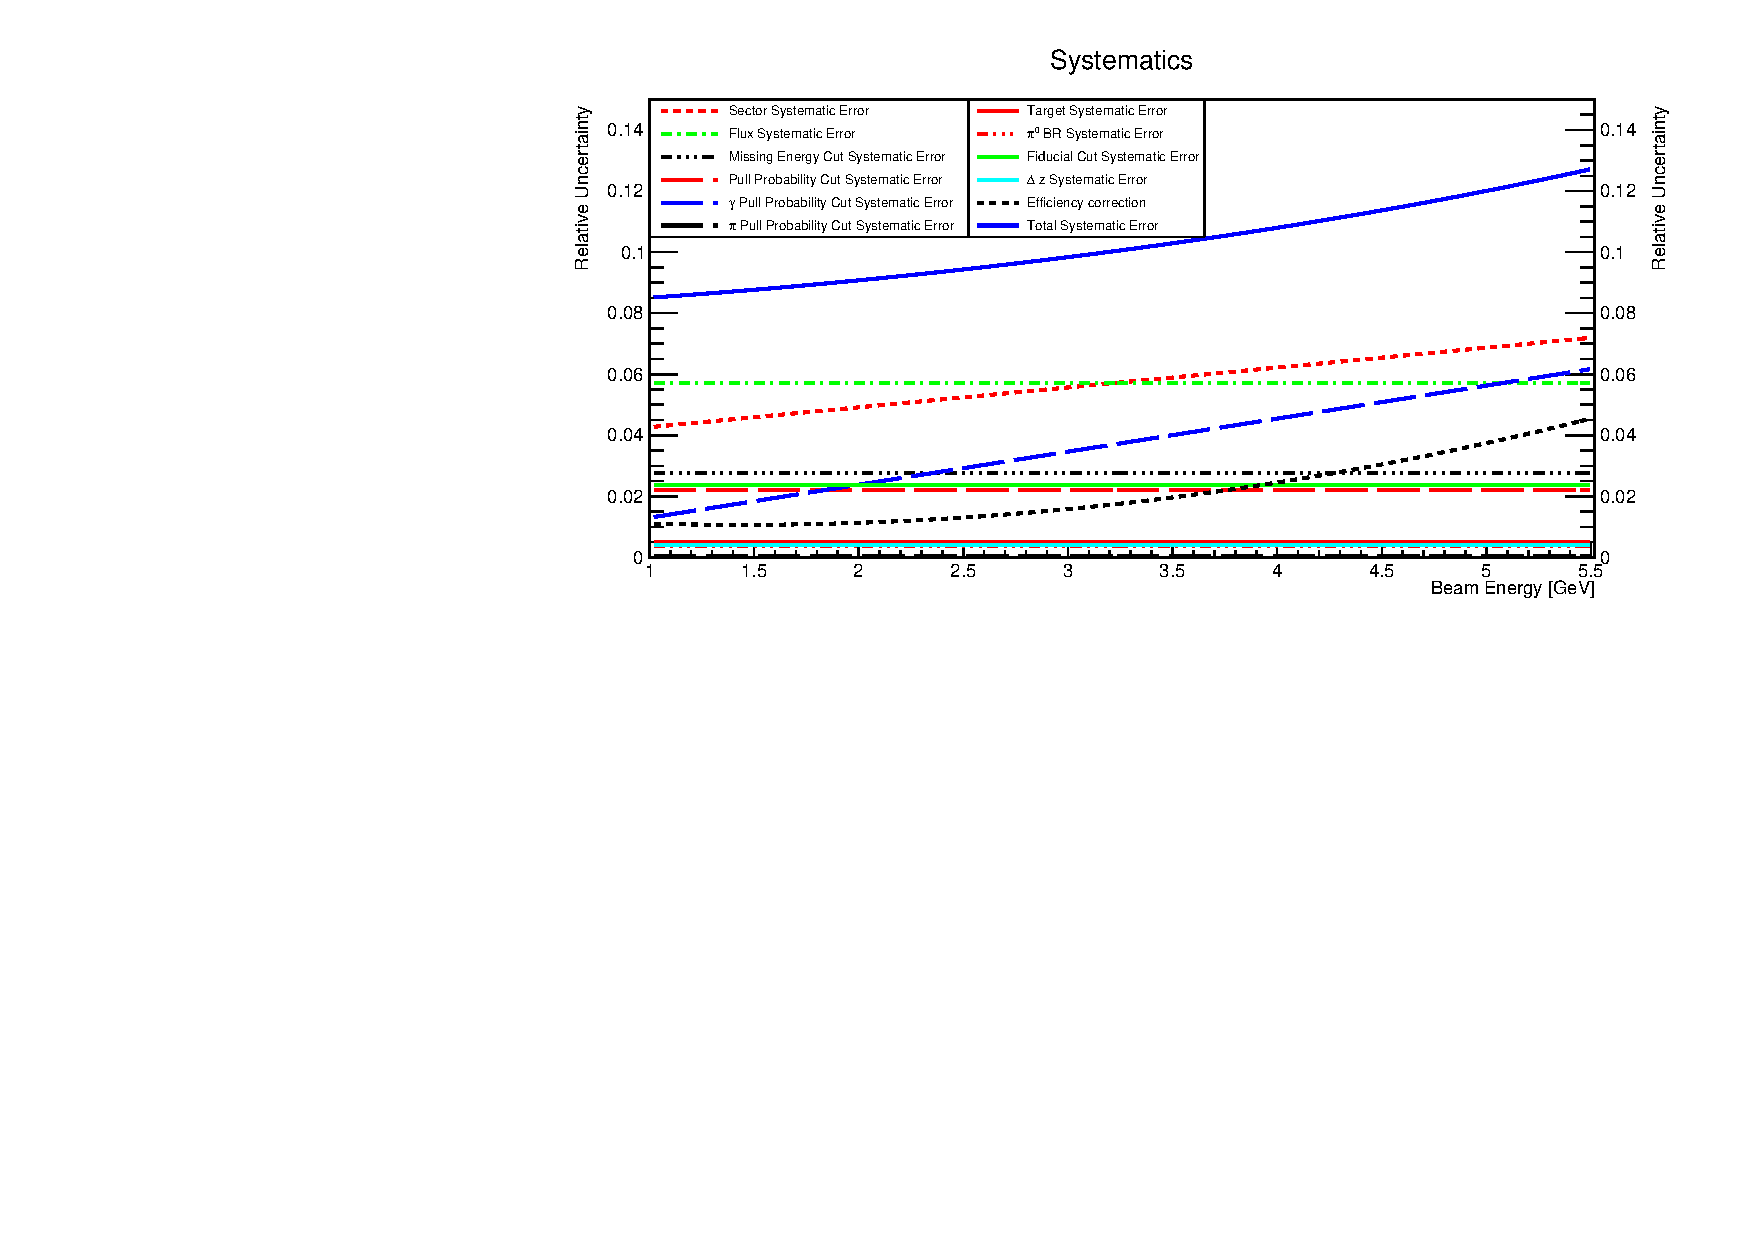
\includegraphics[width=1.0 \figwidth,height=0.9\hfigheight]{/Users/michaelkunkel/WORK/CLAS/CLAS6/CODES/SVN/clas/PI0/SYSTEMATIC/TOTAL_SYSTEMATICS/All_Systematics.pdf}
		\caption{Relative error difference between the two sets of track efficiencies uncertainties reported.}\label{fig:toteff_sys}
	\end{center}\end{figure}
	
	
\begin{figure}[h!]\begin{center}
		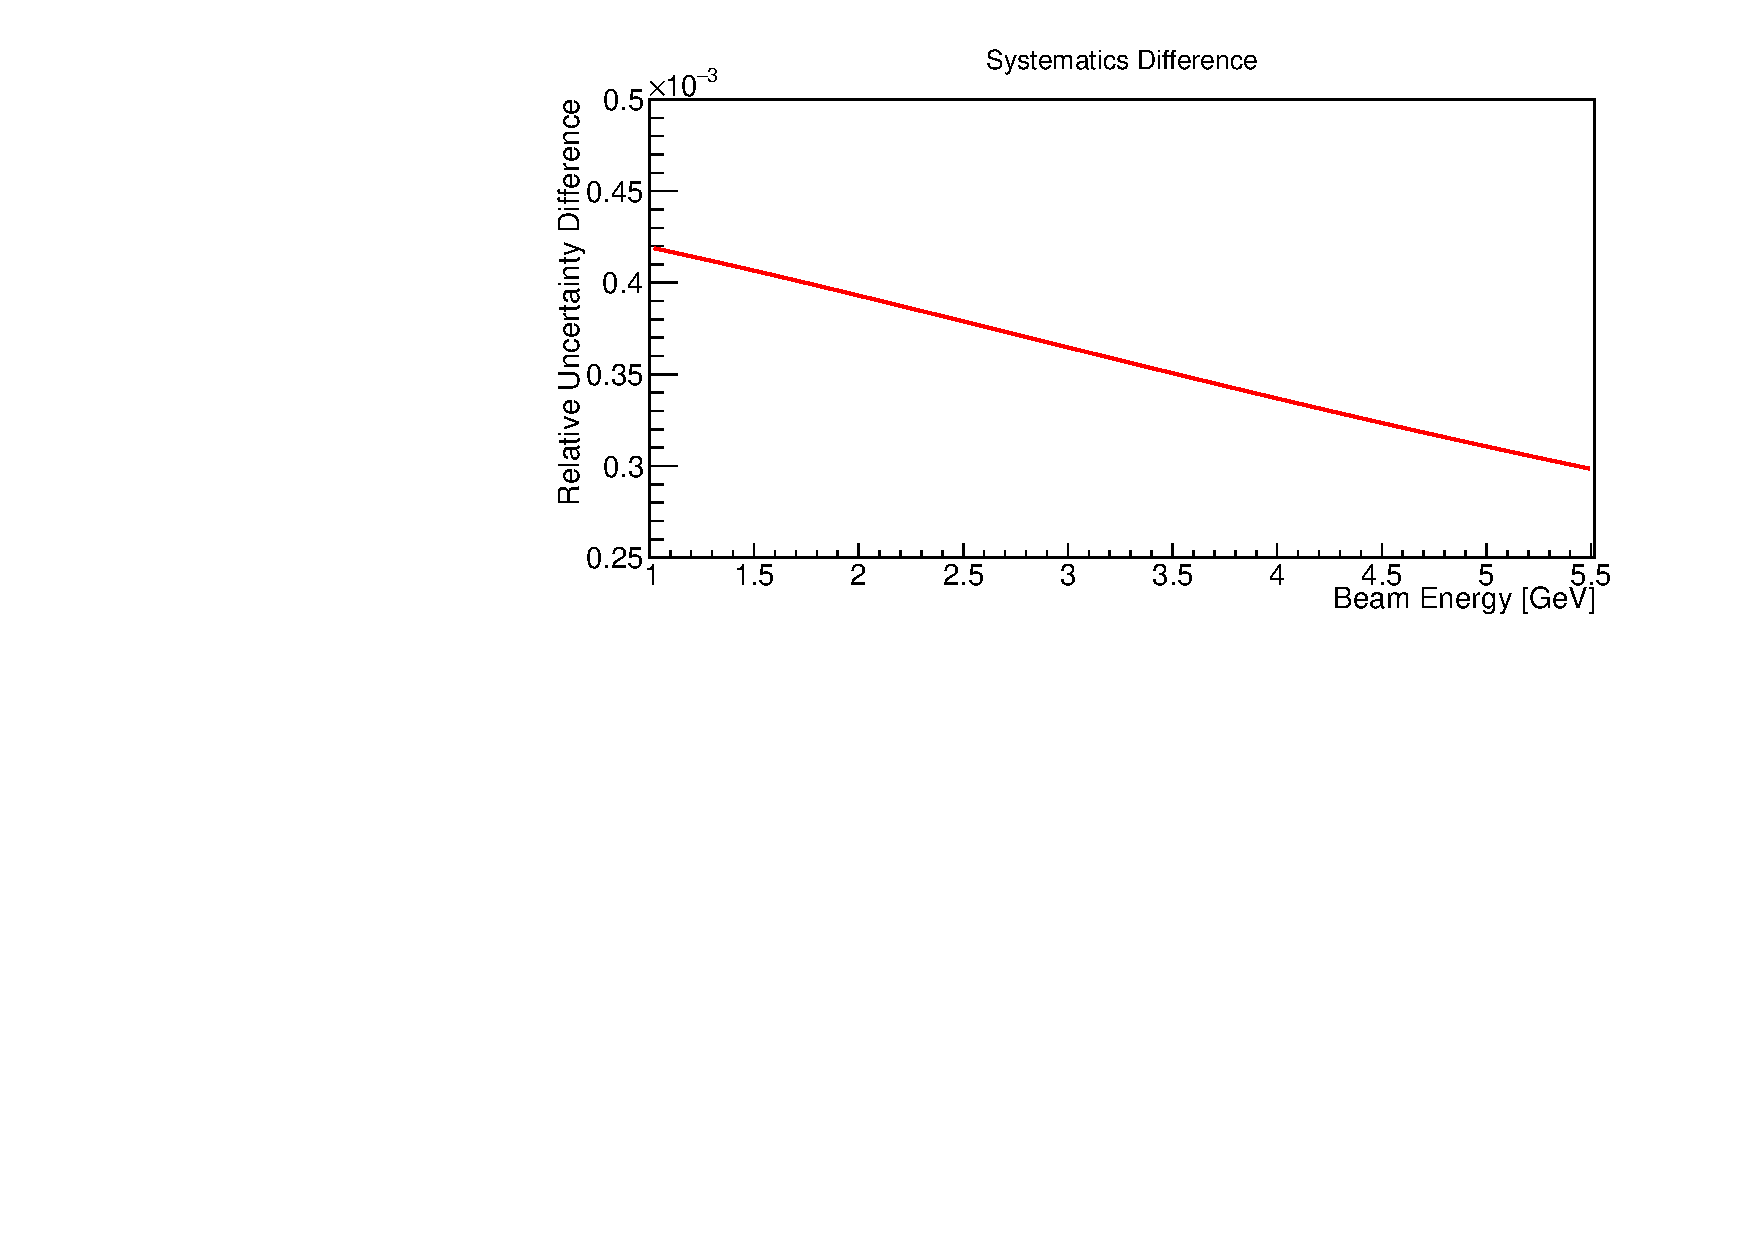
\includegraphics[width=1.0 \figwidth,height=0.9\hfigheight]{/Users/michaelkunkel/WORK/CLAS/CLAS6/CODES/SVN/clas/PI0/SYSTEMATIC/TOTAL_SYSTEMATICS/All_SystematicsDiff.pdf}
		\caption{Relative error difference between the two sets of track efficiencies uncertainties reported.}\label{fig:toteff_DIFF}
\end{center}\end{figure}
\end{document}